% Generated by scripts/make_figures.py.
% Source: experiments/000-repro-baseline/TOLERANCE.md section 3.
\begin{figure}[t]\centering
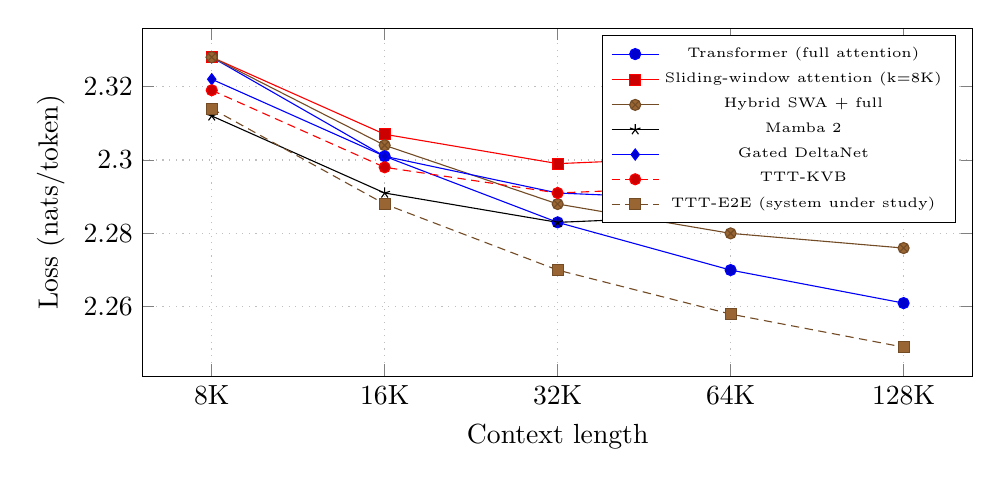
\begin{tikzpicture}
\begin{semilogxaxis}[width=\columnwidth,height=6cm,log basis x=2,
  xtick={8,16,32,64,128},xticklabels={8K,16K,32K,64K,128K},
  xlabel={Context length},ylabel={Loss (nats/token)},
  legend style={font=\tiny,at={(0.98,0.98)},anchor=north east},
  grid=both,grid style={dotted}]
\addplot coordinates {(8,2.328) (16,2.301) (32,2.283) (64,2.270) (128,2.261)}; \addlegendentry{Transformer (full attention)}
\addplot coordinates {(8,2.328) (16,2.307) (32,2.299) (64,2.301) (128,2.309)}; \addlegendentry{Sliding-window attention (k=8K)}
\addplot coordinates {(8,2.328) (16,2.304) (32,2.288) (64,2.280) (128,2.276)}; \addlegendentry{Hybrid SWA + full}
\addplot coordinates {(8,2.312) (16,2.291) (32,2.283) (64,2.285) (128,2.293)}; \addlegendentry{Mamba 2}
\addplot coordinates {(8,2.322) (16,2.301) (32,2.291) (64,2.289) (128,2.295)}; \addlegendentry{Gated DeltaNet}
\addplot coordinates {(8,2.319) (16,2.298) (32,2.291) (64,2.293) (128,2.305)}; \addlegendentry{TTT-KVB}
\addplot coordinates {(8,2.314) (16,2.288) (32,2.270) (64,2.258) (128,2.249)}; \addlegendentry{TTT-E2E (system under study)}
\end{semilogxaxis}
\end{tikzpicture}
\caption{Held-out Books loss against context length for seven
long-context methods. TTT-E2E is lowest at every context length; SWA,
Mamba~2, Gated DeltaNet and TTT-KVB all worsen past 32K.}
\label{fig:baselines}
\end{figure}
